\section{Durchführung}
\label{sec:Durchführung}
Die Messungen werden mit einem D8-Labor-Diffraktometer von Bruker AXS durchgeführt. 
Das Diffraktometer beinhaltet einen Probentisch, eine Röntgenröhre, die Kupfer als Anode verwendet, und einen Detektor.
Letzte zwei können um die Probe rotiert werden. 
Der Probentisch kann in drei Richtungen verschoben werden, um die Probe in den Strahlengang zu bringen.
Die Röntgenröhre operiert mit einer Spannung von $\SI{40}{\kilo\volt}$ und einem Strom von $\SI{35}{\milli\ampere}$.
Zur Bedienung des Diffraktometers und zur Aufnahme der Messwerte wird das Programm \textit{XRD Commander} verwendet.

\subsection{Justage}
\label{subsec:Justage}
\begin{table}[h!]
    \centering
    \begin{tabular}{lccc}
        \toprule
        \textbf{Typ} & \textbf{Messbereich $[^\circ]$} & \textbf{Schrittgröße $[^\circ]$} & \textbf{Messdauer pro Messpunkt [s]} \\
        \midrule
        Detector scan & -0.5 to 0.5 & 0.02 & 1 \\
        Z-Scan & -1 to 1 & 0.04 & 1 \\
        X-Scan & -20 to 20 & 1 & 1 \\
        Rockingscan $\theta = 0$ & -1 to 1 & 0.04 & 1 \\
        Z-Scan & -0.5 to 0.5 & 0.02 & 1 \\
        Rockingscan $\theta = 0.3$ & 0 to 0.3 & 0.005 & 1 \\
        Z-Scan $\theta = 0.3$ & -0.5 to 0.5 & 0.02 & 1 \\
        Rockingscan $\theta = 0.5$ & 0.2 to 0.5 & 0.005 & 1 \\
        \bottomrule
    \end{tabular}
    \caption{Messbereich und Einstellungen für die Justage.}
    \label{tab:Justage1}
\end{table}
Vor der eigenlichen Messung wird das Diffraktometer justiert.
Die für die Justage wichtigen Werte sind in der Tabelle \ref{tab:Justage1} aufgeführt.

Um die Nullposition des Detektors zu bestimmen, wird ein Detektor-Scan durchgeführt.
Dabei rotiert der Detektor um einem kleinen Winkelbereich um die rwartete Nullposition des Röntgenstrahls.
Das Ergebnis des Detektor-Scans liefert eine Gaussförmige Kurve.
Das Maximum des Detektor-Scans wird als neue Nullposition festgelegt.
Die Z-Koordinate der Probe wird durch einen ersten Z-Scan so bestimmt, dass die Probe die halbe Strahlintensität abdeckt.
Dabei wird während des Z-Scans die Z-Koordinate der Probe variiert und die Intensität des reflektierten Strahls gemessen.
Eine schematische Darstellung des Z-Scans ist in Abbildung \ref{fig:zscan} zu sehen.
\begin{figure}[H]
    \centering
    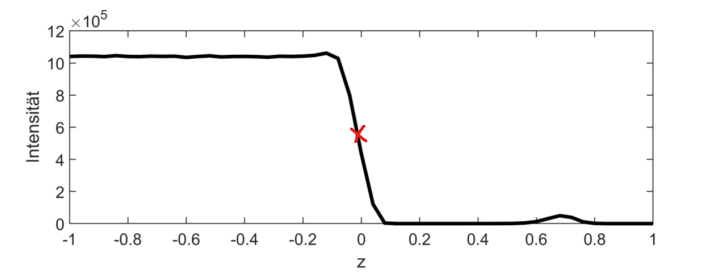
\includegraphics[width=\textwidth]{Bilder/zscan.png}
    \caption{Schematische Darstellung des Z-Scans mit Markierung der optimalen Z-Koordinate \cite{sample}.}
    \label{fig:zscan}
\end{figure}
Um die X-Koordinate der Probe zu bestimmen, wird ein X-Scan durchgeführt.
Hierbei wird die X-Koordinate der Probe variiert und die Intensität des reflektierten Strahls gemessen.
Der durchgeführte Scan weist ein Plateau mit geringerer Intensität auf, innerhalb welches die Probe platziert wird.
Zusätzlich wird ein Rockingscan durchgeführt, um die Probe parallel zum Strahl auszurichten.
Beim Rockingscan rotieren die Röntgenröhre und der Detektor um die Probe.
Die Y-Koordinate wird angepasst, bis der Rockingscan ein symmetrisches Ergebnis liefert.
Das Maximum des Rockingscans gibt die Postion der Probe für eine parallele Ausrichtung an.
Durch die Neigung der Probe muss ein weiterer Z-Scan durchgeführt werden, um die Probe erneut so zu positionieren, dass sie die halbe Strahlintensität abdeckt.
Diese Schritte werden für die Winkel $2 \theta = 0.3$ und $2 \theta = 0.5$ wiederholt, um eine optimale Justage zu erreichen.

\subsection{Messung der Reflektivität eines polymerbeschichteten Silizium-Wafers}
\label{subsec:Messung}
Für die Messung der Reflektivität eines polymerbeschichteten Silizium-Wafers wird ein Omega/2Theta-Scan durchgeführt.
Der Winkebereich beträgt $0^\circ$ bis $2.5^\circ$, mit einer Schrittweite von $0.005^\circ$ und einer Messdauer von $\SI{5}{\second}$ pro Messpunkt.
Bei dieser Messung ist der Einfallswinkel zwischen der Probe und dem Strahl gleich dem Ausfallswinkel zwischen der Probe und dem Detektor.
Um die diffuse Strahlung zu messen, wird die gleiche Messung durchgeführt, allerdings wird der Detektorwinkel um $2^\circ$ verschoben.